\documentclass[11pt,a4paper]{article}
%\usepackage{tkz-orm}

\typeout{------------------------------------------------------------------}
\typeout{} 
\typeout{        Fichier de base modifie par : Matth: 20 nov 2012} 
\typeout{                   sous licence GNU-GPL} 
\typeout{}
\typeout{------------------------------------------------------------------}

% Classe générale du document
   %documentclass[12pt,a4paper]{article} % .10pt, 11pt, 12pt : taille de la police principale (10 par défaut)
                 % .a4paper, letterpaper,... : délimite la taille du papier. (letterpaper par défaut)
	         % .fleqn : aligne les formules mathématiques à gauche au lieu de les centrer.
		 % .leqno : place la numérotation des formules à gauche plutôt qu'à droite.
		 % .twocolumn : demande à LATEX de formater le texte sur deux colonnes.
		 % .twoside, oneside indique si la sortie se fera en recto-verso ou en recto simple.
		 % .landscape, mais il faut mettre en commentaire (ou modifier) toutes les dimmensions

% Importation de packages divers
%   \NeedsTeXFormat{LaTeX2e} 
   \usepackage[T1]{fontenc}
   \usepackage[utf8x]{inputenc}		% utilisation des caractères 8 bits en Unix (codage ISO 8859-1)
  %\usepackage[latin1]{inputenc}	% utilisation des caractères pour Linux2
   \usepackage[usenames]{color}
   \usepackage{fancyhdr}
   \usepackage{lastpage}                % pour l'affichage du n° de la dernière page.
   \usepackage{lmodern}
   \usepackage{multirow}                % pour l'utilisation de figures ``noyées'' dans le texte
   \usepackage{xspace}			% package pour babel
   \usepackage[english]{babel}         % Utilisation du français (nom des sections, césure, ponctuation,...)
   \usepackage[english]{varioref}        % vpageref
   \usepackage{amsmath,amsthm,amssymb}  % Utilisation de certains packages de AMS (cf. belles équations)
   \usepackage{endnotes}                % Pour l'utilisation des notes en fin de documents
   \usepackage{verbatim}                % Pour l'insertion de fichier en mode verbatim
   \usepackage{portland}		% pour l'utilisation de \portrait et de \landscape sur une page
   \usepackage[pdftex]{graphicx}        % [pdftex] si utilisation d'images jgp,...
                                        % [dvips]  si utilisation d'images bmp,...
   \usepackage{pdfpages}		% Inclure des pages de pdf
   \usepackage{pdflscape}		% rotate => begin{landscape} ... \end{landscape}
   \usepackage{setspace}		% Pour définir un interligne
   \usepackage{tkz-orm}
   \usepackage[bottom]{footmisc}        % Footnote at the bottom
%   \usepackage[cyr]{aeguill}		% Pour les guillemets à la Française
   \usepackage{eurosym}			% Pour les Euro
   \usepackage{url}
    \urlstyle{sf}
   \usepackage[backgroundcolor=yellow]{todonotes} %% todonotes: \listoftodos & \todo{Some note or other.} & \missingfigure{}
	
   \renewcommand{\contentsname}{Sommaire} % si tableofcontents au début
   \newcommand{\Numero}{\No}
   \newcommand{\numero}{\no}
%   \newcommand{\fup}[1]{\up{#1}}

   \DeclareGraphicsExtensions{.jpg,.pdf,.mps,.png}       % déclaration d'extensions  pour les images
   %\input xy                            % pour le package xy (construction de diagramme)
   %\xyoption{all}

% Dimensions de la page :       	

  %%%%%%%%%%%%%%%%%%%%%%%%%%%%%%%%%%%%%%%%  0
  %   |                                  %
  %---+----------------------------------%  1
  %   | +----------------------------+   %  2
  %   | |          en-tête           |   %
  %   | +----------------------------+   %  3
  %   | +----------------------------+   %  4
  %   | |                            |   %       Remarques : 
  %   | |                            |   %        . distance de '0' à '1' : un pouce + \voffset
  %   | |                            |   %        . distance de 'a' à 'b' : un pouce + \hoffset
  %   | |           texte            |   %
  %   | |                            |   %
  %   | |                            |   %
  %   | |                            |   %
  %   | +----------------------------+   %  5
  %   | +----------------------------+   %
  %   | |         bas de page        |   %
  %   | +----------------------------+   %  6
  %%%%%%%%%%%%%%%%%%%%%%%%%%%%%%%%%%%%%%%%
  %a  b c                            d  e

%    % général
%      \voffset       0mm    % pour descendre (si positif) ou remonter (si négatif) le tout
%      \hoffset       0mm    % pour agrandir (si positif) ou diminuer (si négatif) la marge gauche (distance 'a' 'b')
%      \oddsidemargin 0mm   % 5pt  % distance de 'b' à 'c'
%     \evensidemargin 25mm  % 15pt % distance de 'd' à 'e'
%    % texte
%      \headsep       25pt   % distance de '3' à '4', la distance entre l'en-tête et le texte
%     \textheight    220mm  % distance de '4' à '5', pour déterminer la hauteur du texte
%     \textwidth     160mm  % distance de 'c' à 'd' 
%    % en-tête
%     \topmargin     0pt    % distance de '1' à '2', pour descendre (si positif) ou remonter (si négatif) le tout
%     \headheight    15pt   % distance de '2' à '3', doit être > 14.49999
%    % bas de page
%     \footskip      15mm   % 30pt % distance de '5' à '6', la distance entre le texte et le bas de page
     % space for the footnode
%    \setlength{\skip\footins}{1cm}

\usepackage[top=2.5cm, bottom=2.5cm, left=2.5cm, right=2.5cm]{geometry}

% (Re)définitions diverses

  % redéfinition de l'affichage des titres de section dans l'en-tête ou le bas de page
    % remarques :
    %  .affichage du numéro (2)    : \thesection 
    %  .affichage du nom (Section) : \sectionname
   % \renewcommand{\sectionmark}[1]{\markright{\thesection.\ #1}}   % 2.2. nom de la section 2.2
   % \renewcommand{\thesection}{\arabic{section}}		% II nom de la section 0.2


  % des couleurs...                   (utilisation avec par ex. \textcolor{webdarkblue}{...})
   \definecolor{codeBlue}{rgb}{0,0,1}
   \definecolor{webred}{rgb}{0.5,0,0}
   \definecolor{codeGreen}{rgb}{0,0.5,0}
   \definecolor{codeGrey}{rgb}{0.6,0.6,0.6}
   \definecolor{webdarkblue}{rgb}{0,0,0.4}
   \definecolor{webgreen}{rgb}{0,0.3,0}
   \definecolor{webblue}{rgb}{0,0,0.8}
   \definecolor{orange}{rgb}{0.7,0.1,0.1}

  % utilisation de caption, label,... pour autre chose qu'une figure
        %%%% debut macro %%%%
   \makeatletter
   \def\captionof#1#2{{\def\@captype{#1}#2}}
   \makeatother
        %%%% fin macro %%%%


% remarques : 
%  . pour mettre la date                  : \today
%  . pour mettre le nom de la section     : \rightmark
%  . pour mettre le numéro de page        : \thepage
%  . pour mettre le nombre de pages total : \pageref{LastPage}  (mais l'écrit en rouge vu que c'est une réf.)
%  . insertion d'une image                : \setlength{\unitlength}{1mm}
%                                             \begin{picture}(0,0)
%                                                \put(5,0){\includegraphics[scale=x.x]{xxx.xxx}}
%                                             \end{picture}

% Pour les guillemets à  la Française
\newcommand{\fermerguillemets}{\unskip\kern.15em\symbol{20}}
\newcommand{\ouvrerguillemets}{\symbol{19}\ignorespaces\kern.15em}
% \let »=\fermerguillemets
% \let« =\ouvrerguillemets

% Pour changer l'icone des puces : à placer juste avant une liste
 %   \renewcommand\labelitemi{\textbullet}	% Style boulet :)
\usepackage[pdfusetitle,
	    colorlinks=true,
	    linkcolor=webdarkblue, 
	    filecolor=webblue, 
	    urlcolor=webdarkblue,
	    citecolor=webgreen]{hyperref}     % pour l'utilisation des liens http,...

% Police
   %\renewcommand\familydefault{ptm}        % famille normale: Times ptm
   %\renewcommand\rmdefault{phv}            % famille à utiliser pour du Roman (phv)
   \renewcommand{\familydefault}{\sfdefault}

% L'interligne
%   \onehalfspacing % un et demi (= \setstrech{1.5} ou = \renewcommand{\baselinestretch}{1.5})
%   \renewcommand{\baselinestretch}{1.15}

     
% Mise en page
%   \pagestyle{fancy} %% custom en-tête
%   \usepackage[Matth]{fncychap}

% En-tete
%   \lhead{\texttt{LECGE1321} - Travail de Management Humain}        \chead{}        \rhead{Groupe 74}
%   \renewcommand{\headrulewidth}{0.5pt}     % pour l'épaisseur de la ligne

% Bas de page
%   \renewcommand{\footrulewidth}{0.5pt}       % pour l'épaisseur de la ligne
%   \lfoot{Partie \rightmark}        \cfoot{}        \rfoot{Page \thepage~sur~\pageref*{LastPageModif}}

% TOC jusqu'au subsection
\setcounter{tocdepth}{2} % Dans la table des matieres
\setcounter{secnumdepth}{3} % Avec un numero.

\usepackage{listings}
\lstset{
    language=Ruby,
	breakatwhitespace=true,
	breaklines=true,
	keepspaces=true,
	numbers=left,
	numbersep=5pt,
	showstringspaces=true,
	frame=single,
	basicstyle=\footnotesize,
	title=\lstname,
    literate=
      {á}{{\'a}}1 {é}{{\'e}}1 {í}{{\'i}}1 {ó}{{\'o}}1 {ú}{{\'u}}1
      {Á}{{\'A}}1 {É}{{\'E}}1 {Í}{{\'I}}1 {Ó}{{\'O}}1 {Ú}{{\'U}}1
      {à}{{\`a}}1 {è}{{\'e}}1 {ì}{{\`i}}1 {ò}{{\`o}}1 {ò}{{\`u}}1
      {À}{{\`A}}1 {È}{{\'E}}1 {Ì}{{\`I}}1 {Ò}{{\`O}}1 {Ò}{{\`U}}1
      {ä}{{\"a}}1 {ë}{{\"e}}1 {ï}{{\"i}}1 {ö}{{\"o}}1 {ü}{{\"u}}1
      {Ä}{{\"A}}1 {Ë}{{\"E}}1 {Ï}{{\"I}}1 {Ö}{{\"O}}1 {Ü}{{\"U}}1
      {â}{{\^a}}1 {ê}{{\^e}}1 {î}{{\^i}}1 {ô}{{\^o}}1 {û}{{\^u}}1
      {Â}{{\^A}}1 {Ê}{{\^E}}1 {Î}{{\^I}}1 {Ô}{{\^O}}1 {Û}{{\^U}}1
      {œ}{{\oe}}1 {Œ}{{\OE}}1 {æ}{{\ae}}1 {Æ}{{\AE}}1 {ß}{{\ss}}1
      {ç}{{\c c}}1 {Ç}{{\c C}}1 {ø}{{\o}}1 {å}{{\r a}}1 {Å}{{\r A}}1
      {€}{{\EUR}}1 {£}{{\pounds}}1
}


% Juste pour avoir un titre dans le pdf
\title{Software Development Project - Report 3}
\author{Group 6: Matthieu Baerts, Benoît Baufays, Julien Colmonts, Benjamin Frantzen, Pierre-Yves Légéna, Vincent Van Ouytsel, Ludovic Vannoorenberghe, Alex Vermeylen}

\begin{document}

% \listoftodos %% TODO %% REMOVE %%%%%%%%%%%%%%%%%%%%%%%%%%%%%%%%%%%%%%%

\begin{titlepage}
\newgeometry{left=2cm,right=2cm,top=2cm,bottom=2cm}

\rm %% style Roman for the title

\begin{center}

% Upper part of the page
%\vspace*{-2cm}
\includegraphics[scale=.5]{ingi.png}\\[2cm]

\textsc{\LARGE Pôle d'ingénierie informatique}\\[1.5cm]

\textsc{\Large \texttt{LSINF2255} - Software Development Project}\\[0.5cm]


% Title
\vspace{3.5cm}
{ \huge \bfseries Design analysis report\vspace{0.8cm}}

\vspace{3.5cm}

% Author and supervisor
\begin{minipage}{0.4\textwidth}
\begin{flushleft} \large
\emph{Professor:}\\
	Kim \textsc{Mens}\\
\vspace{1cm}
\emph{Assistant:}\\
	Sergio \textsc{Castro Mejia} % Apple lover
\end{flushleft}
\end{minipage}
\begin{minipage}{0.4\textwidth}
\begin{flushright} \large
\emph{Students: (Group 6 - SINF2MS)} \\
%\begin{tabular}{rr}
	Matthieu \textsc{Baerts}\\
	Benoît \textsc{Baufays}\\
	(\textit{Project Manager}) Julien \textsc{Colmonts}\\
	Benjamin \textsc{Frantzen}\\
	Pierre-Yves \textsc{Légéna}\\
	Vincent \textsc{Van Ouytsel}\\
	Ludovic \textsc{Vannoorenberghe}\\
	Alex \textsc{Vermeylen}
%\end{tabular} \\
\end{flushright}
\end{minipage}

\vfill

% Bottom of the page
{\large Academic Year 2013-2014}
\end{center}

\end{titlepage}
\restoregeometry

\tableofcontents
\thispagestyle{empty}	% pour enlever le numéro de page
\newpage
\pagenumbering{arabic} % on triche avec la numéroation des pages :)

\section*{Introduction}
\addcontentsline{toc}{section}{Introduction}
% intro ~ok


In this first report, we describe the first step of our development project following the waterfall model: the requirements. It means that we have listed all features that will be implemented in our project. This will be done by taking into account the different users that might use the system. All actions that users want to find on our website are listed as user stories.

We have analysed the requirements and used them to draw activity diagrams and to write user stories to show up the main functions of our website. The activity diagrams are graphical tools showing interactions between a user and the application we have to design. A user story is a kind of scenario that a user of the system does or needs to do.\\

In addition to that, we also enumerate a few non-functional requirements that describe how the system should handle all the functionalities.

\section{UML Classes Diagram}
After the architectural report, we took in consideration the remarks pointed by our teacher and his assistant. We updated it to correct relations between objects. \\

\subsection{UML Class diagram}

\begin{figure}[!ht]
	\begin{center}
		\includegraphics[width=\textwidth]{UML.png}
		\caption{Unified Modeling Language (UML): class diagram, model. This figure is also visible in a bigger size in the appendix, figure \vref{fig:uml_big}}
		\label{fig:uml}
	\end{center}
\end{figure}

Our diagram can be divided in three parts. The first part, on the left, shows the organisation part of the model. The organisation object has a name and contains some addresses (an organisation can have multiple contact points), some co-workers, managed users and created services by its users. This last link, between an organisation and a service, is absolutely not mandatory; it exists only if the service is created by a co-worker for a managed user. The co-workers are working for a single organisation for some users. They are modelled by an extension of a user because they will have an account to log in and they will be able to create services, even if it's for other users.\\

The second part, on the center of the diagram, is dedicated to the users. A main user is defined as an abstract user and contains all the informations that are in common for each kind of users. The application will be used by five kinds of users, directly or indirectly. The most common one is defined as a simple user. A user that will connect to the application from his home, sign in and he's ready to offer or demand services. This kind of account needs an e-mail verification and a password to connect to. Extension of this kind of user can be divided in two groups, the coworkers of an organisation and the administrators of the website. We already talked about coworkers a few lines above. For administrators, there are two level of responsibilities. First level is for moderators who will be able to manage services from the categories they are bound to. This choice is made to restrict responsibilities to some categories for a single administrator. The more powerful administrators stand at level 2. They are able to accept organisation registrations and manage users account (delete them if they don't respect the website policies). Notice that a user can have multiple addresses, it's a choice led by the idea of helping users to show different places where the service can be delivered. \\

The third part, on the right, explains the service part of the model. As for the users, we created an abstract part for services containing the object common parameters. A service is related to several subcategories to help user in his searches. In the same philosophy as we saw on websites like \textit{eBay}, we divided categories in subcategories. For example, a demand asking for clothes can be more detailed in specifying what kind of clothes the user wants (like winter clothes, summer clothes,etc.). Extensions of the abstract class are the specific kind of services : offers and demands. They are regrouped after a match in an object called transaction that will contains feedback from both users. You can see that we added a boolean \texttt{Quick} field in the service object. It's used to point a service that's created for a manual matching. For example, a user accepts an offer without having created a demand which match this offer. The  matching demand creation for registering the transaction in the database will not appear to the user.\\

Since we have more experiences in Java programming, we are used to design class diagrams with abstract classes. In Ruby, using abstract classes isn't as usual than in Java, and a bit harder to implement. We'll maybe define these objects as standard objects but we'll never instantiate them.\\
\begin{figure}[!ht]
	\begin{center}
		\includegraphics[width=.8\textwidth]{UML_Controller.png}
		\caption{Unified Modeling Language (UML): class diagram, controller.}
		\label{fig:uml_controller}
	\end{center}
\end{figure}

In an effort of completeness, we made a controller class diagram related to all methods and functions written in the sequence diagrams that are shown below. There are no relation between them because Rails manages these relations on his own. The application controller is the main one with most responsibilities. 

\subsection{Sequence diagrams}

\begin{figure}[!ht]
	\begin{center}
		\includegraphics[scale=.5]{dubble_arrow.png} %% 75
		\caption{A double arrow is used to indicate an action of routing}
		\label{fig:darrow}
	\end{center}
\end{figure}
In the following diagrams, we decided to use the double arrow (like the one on figure \vref{fig:darrow}) to indicate an action of routing. It means that in the entry point of a diagram a user has been redirected to this page. Or at a moment of the diagram after some actions the user is redirect somewhere else on the website.

\texttt{current\_user} is a global variable which represents the user who is actually connected. The default value, when no user is connected, is \texttt{NULL}.

Another convention is \texttt{params*}. It represents all the parameters given by the form when we create an object like a user or a service.

\subsubsection{Log-in}

\begin{figure}[H]
	\begin{center}
		\includegraphics[width=.45\textwidth]{log_in.png} %% 70
		\caption{Sequence Diagram: Log-in}
		\label{fig:login}
	\end{center}
\end{figure}

This scheme modeles the action sequence when a user try to log in. As we can see, we check in
the database if this user exist. To do this we make a request that returns a \texttt{User} object. If
the user doesn't exist in the database, then this object is \texttt{NULL}. In this case,
we redirect the user to the log in page of the website ; otherwise, we connect to the profile and the current user is updated.

\subsubsection{User account creation}

\begin{figure}[H]
	\begin{center}
		\includegraphics[width=.7\textwidth]{user_new.png} %% 100
		\caption{Sequence Diagram: User account creation}
		\label{fig:newuser}
	\end{center}
\end{figure}

To create a new user, we first have to check if the user is not already connected. If it is and if it's
not an organisation, then we redirect him to the root page because an already connected user cannot 
create a new account. In the case of an organisation, it is of course possible 
for it to create new users. Then, if no error occurs, we create a new \texttt{User} and we update its field \texttt{id\_orga}. This fields can contains \texttt{NULL} if the user creates his account on his own purpose or the id of the organisation that created for him. Then the user is added to the
database which send a response containing  possible error if the user already exists in the database.

\subsubsection{Search}

\begin{figure}[H]
	\begin{center}
		\includegraphics[width=.55\textwidth]{search_a_service.png} %% 80
		\caption{Sequence Diagram: Search a service}
		\label{fig:searchservice}
	\end{center}
\end{figure}

In this case, we show how the result of a search is proceeded. In the case where \texttt{params*} is \texttt{NULL}, we ask the database manager to return the ten last services (in a table \texttt{Service[]}) added to the platform ;
otherwise, we look at the database to do a match between the requested service represented by informations in the \texttt{params*} and the services that are available in the database. Finally the database manager sent an array of services containing either the "top ten" or the matching services.
Our extension is the advanced search.  To do that, we choose to change only the match method.  Then, the information in the \texttt{params*} change regarding the search we just made. 
\\If the client want to do more precise researches, we'll filter the results of the search on the client side. With this solution, we'll do less requests on the server.

\subsubsection{Service creation}

\begin{figure}[H]
	\begin{center}
		\includegraphics[width=.75\textwidth]{service_new.png} %% 100
		\caption{Sequence Diagram: Service creation}
		\label{fig:newservice}
	\end{center}
\end{figure}

We'll describe here the creation of a service. First, we check if the user is connected. If he is not, we redirect the user to the main page ; otherwise, we create a service object and we update its \texttt{id\_creator} field with 
the id of the current user. Then we save the service in the database. Finally, we redirect the user to a page displaying the result of a search with the newly created service.


\subsubsection{Service acceptance}
\begin{figure}[H]
	\begin{center}
		\includegraphics[width=.70\textwidth]{service_accepted.png} %% 95
		\caption{Sequence Diagram: Acceptance of an offer or a demand, visible in a bigger size in the appendix, figure \vref{fig:acceptService_big}}
		\label{fig:acceptService}
	\end{center}
\end{figure}

This scheme shows what happens when a service is accepted. First, we check if the user is connected.
If not, we redirect him to the home page. 
Then we proceed a \texttt{best\_match\_search} which returns all the services which match the request of the user.
If there are no result, we create a \texttt{Quick Service} which perfectly matches the user's expectation.

\subsubsection{End of service}
\begin{figure}[H]
	\begin{center}
		\includegraphics[width=.9\textwidth]{end_of_service.png}
		\caption{Sequence Diagram: End of a transaction}
		\label{fig:end_of_service}
	\end{center}
\end{figure}

When the creator and the customer have met and proceed the service, they can add a feedback for it.
When the creator or the customer do that, he fills a form (\texttt{params*} field on the figure below).  The route (\texttt{service\#finished}) is catching by the \texttt{ServiceController} and it creates a new transaction with the \texttt{params*} and the \texttt{current\_user}.
After that, we must update the karma of the other user that perform the service. The karma of the current user will be updated as well by the other
user.
Finally, we show the feedbacks page of the \texttt{current\_user}.

\subsubsection{Validation with the identity card}
\label{SEC:valid_ID}
\begin{figure}[H]
	\begin{center}
		\includegraphics[width=1\textwidth]{check_ID.png}
		\caption{Sequence Diagram: Certifying a user by using the identity card}
		\label{fig:eID}
	\end{center}
\end{figure}

This diagram shows how the user can validate his account. After having received the signature, the \texttt{UserController} will use the \texttt{eIDController} to contact the authority in order to know if the signature is valid or not. If it is, the user is certified and we can save this information in the database.\\
At the end of this operation, the user is redirected to his profile page with a confirmation or an error message.\\
You can find this figure in bigger size in the appendix, figure \vref{fig:eID_big}.\\

To test the ID verification, the Belgium government provides a service\footnote{To learn more about that: \url{https://env.dev.eid.belgium.be/testkit.php}} that allow us to generate ID card.
As the ID verification functionality is an advanced properties. It will take lot of time to be developed, so we will implement it only if we have enough time.

\subsubsection{Ban from an Administrator}

\begin{figure}[H]
	\begin{center}
		\includegraphics[width=.55\textwidth]{ban_user.png}
		\caption{Sequence Diagram: Ban a user from the website}
		\label{fig:ban}
	\end{center}
\end{figure}

In this scheme, we show one of the possible actions available to the administrator.
The method \texttt{ban(user\_id)} just check for the user corresponding to the id and edit his \texttt{inscription\_ok} in the database with the \texttt{False} value.


\subsection{Box Pointer Diagram}
 \begin{figure}[H]
	\begin{center}
		\includegraphics[width=.8\textwidth]{boxpointer.png}
		\caption{Box pointer diagram : Overall architecture}
		\label{fig:boxpointer}
	\end{center}
\end{figure}

In the previous report, we put this diagram to show a general overview of how the application should be used. In the feedback, we saw that it wasn't enough explained so we'll bring some additional informations about it. First, there are two databases shown but actually there will be only one in the real application. This was made to show which operation works with which part of the database. You can see this link with the orange arrows. The green arrows show a general flow of using the application in terms of time.


\section{Database relational schema}
\begin{center}
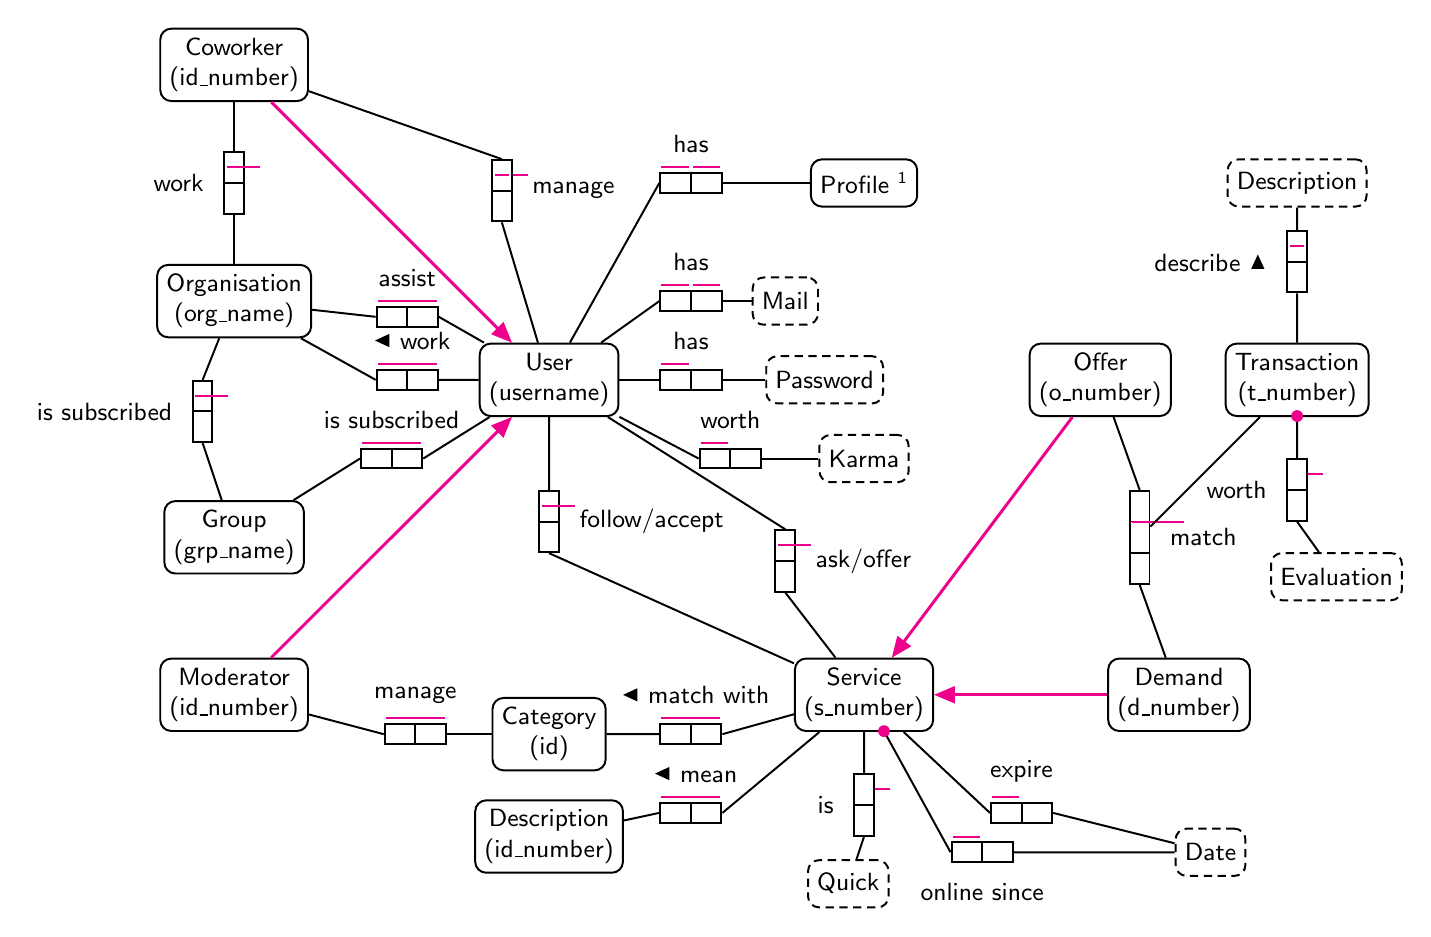
\begin{tikzpicture}[orm]

\entity (U) at (0,0) {User\\(username)};
\entity (Profile) at (4,2.5) {Profile \footnotemark[1]};
\entity (Org) at (-4, 1) {Organisation\\(org\_name)};
\entity (Gr) at (-4,-2) {Group\\(grp\_name)};
\entity (S) at (4, -4) {Service\\(s\_number)};
\entity (O) at (7, 0) {Offer\\(o\_number)};
\entity (D) at (8, -4) {Demand\\(d\_number)};
\entity (T) at (9.5,0) {Transaction\\(t\_number)};
\entity (C) at (0, -4.5) {Category\\(id)};
\entity (Desc) at (0, -5.8) {Description\\(id\_number)};
\entity (Ad) at (-4, -4) {Moderator\\(id\_number)};
\entity (Co) at (-4, 4) {Coworker\\(id\_number)};

\value (M) at (3,1) {Mail};	
\value (Pa) at (3.5,0) {Password};	
\value (K) at (4, -1) {Karma};	
\value (Tdesc) at (9.5, 2.5) {Description};
\value (Teval) at (10, -2.5) {Evaluation};
\value (Date) at (8.4,-6) {Date};	
\value (Quick) at (3.8, -6.4) {Quick};

\binary[right= of U,  unique=1, unique=2, label=has] (h) at (1, 2.5) {};
\binary [right=of U, unique=1, unique=2, label=has] (h2) at (1, 1) {};
\binary [right=of U, unique= 1, label=has] (h3) at (1, 0) {};
\binary [right=of U, unique= 1, label=worth] (h4) at (1.5, -1) {};
\binary [left=of U, unique=1-2, label=assist] (h5) at (-1, 0.8) {};
\binary [left=of U, unique=1-2, label=\ormleft{work}] (h6) at (-1, 0) {};
\vbinary [left=of U, unique=1-2, label=is subscribed] (h7) at (-4, 0) {}; 
\binary [unique=1-2,label=is subscribed] (h8) at (-2,-1){};
\vbinary [unique=1-2,label=below:follow/accept] (h8bis) at (0,-1.8){};
\vbinary [unique=1-2, label=below:ask/offer] (h9) at (3,-2.3) {};
\vternary [unique=1-3, label=below:match] (h10) at (7.5,-2){};
\vbinary [unique=1, label= \ormup{describe}] (h19) at (9.5, 1.5) {};
\vbinary [unique=2, label=worth] (h20) at (9.5, -1.4) {};
\binary [unique=1-2, label=\ormleft{match with}] (h11) at (1.8, - 4.5) {};
\binary [unique=1-2, label=\ormleft{mean}] (h12) at (1.8, - 5.5) {}; 
\binary [unique=1, label=expire] (h13) at (6,-5.5){};
\binary [unique=1, label=below:online since] (h14) at (5.5,-6){}; 
\binary[right= of Ad, label=manage, unique=1-2] (h21) at (-2.5,-4.5) {};
\vbinary[right= of Co, label=below:manage, unique=1, unique=2] (h22) at (-1,2) {};
\vbinary[unique=1-2, label=work] (h23) at (-4, 2.5) {};
\vbinary[unique=2, label=is] (h24) at (4, -5.4) {};
 
\plays  (U) to (h.west) (S) to (h24.east) (h24.west) to (Quick);
\plays (h.east) to (Profile);
\plays (U) to (h2.west); 
\plays (h2.east) to (M); 
\plays (U) to (h3.west); 
\plays (h3.east) to (Pa); 
\plays (U) to (h4.west); 
\plays (h4.east) to (K); 
\plays (U) to (h5.east) (h5.west) to (Org) (U) to (h6.east) (h6.west) to (Org) (Org) to (h7.east); 
\plays (h7.west) to (Gr);
\plays (U) to (h8.east) (h8.west) to (Gr);
\plays (U) to (h8bis.east) (h8bis.west) to (S);
\plays (U) to (h9.east) (h9.west) to (S); 
\plays (O) to (h10.east) (D) to (h10.west) (h10) to (T);
\plays [mandatory] (S) to (h11.east) (S) to (h12.east) (T) to (h19.west) (T) to (h20.east); 
\plays(h11.west) to (C) (h12.west) to (Desc) (h19.east) to (Tdesc) (h20.west) to (Teval);
\plays (S) to (h13.west) (h13.east) to (Date) (h14.east) to (Date);
\plays [mandatory] (S) to (h14.west);

\plays (Ad) to (h21.west);
\plays (h21.east) to (C);
\plays (Co) to (h22.east);
\plays (h22.west)to (U);
\plays (Co) to (h23.east);
\plays (h23.west) to (Org);
 
\draw[subtype] (S) to (O); 
\draw[subtype] (S) to (D); 
\draw[subtype] (U) to (Co); 
\draw[subtype] (U) to (Ad);

\end{tikzpicture}
\end{center}



On the ORM diagram, we added a few elements. First, we added new kinds of \texttt{User}. We did this to show the different kind of users accounts that can be created beside the 'simple user' : \begin{itemize}
\item The \texttt{Coworker}. A user who works for an organisation and can manage different users by creating their account and manage services for them.
\item The \texttt{Moderator}. A user who manages a special category of services.
\end{itemize}
Secondly, we put the new field of service, which is called \texttt{Quick}. It's already explained earlier in this report.


\section{Development plan}
\subsection{Update of the development plan}

As we tried to remain consistent between reports, we see that the development plan doesn't have to change that much.
The way we split the different modules didn't change, neither did the estimated time allocated to each.
Therefore, we send you back there for the Gantt diagram.
The only restriction we'll have is about the validation with the ID card.
As said in section \ref{SEC:valid_ID} the implementation might be quite tricky, so we weren't able to estimate precisely how much time it would need to implement this.
We planned on implementing this along with the \textit{validation} module, but it might take more time.\\

However, we still had to allocate each module to each other.
Here's what we decided :
\begin{itemize}
  \item \textbf{Core Dev}:
  \begin{itemize}
    \item Database: Julien et Benjamin
    \item Model: Matthieu et Benoit
    \item Display: Alex et Ludovic
  \end{itemize}
  \item \textbf{Modules X}:
  \begin{itemize}
    \item Connection/Subscribing system: Vincent et Pierre-Yves
    \item Validation: Alex et Benoit
    \item Account manager: Vincent et Pierre-Yves
    \item Group manager: Alex et Vincent
    \item Organisations: Benjamin et Ludovic
    \item Offer/Demand creator: Julien et Benoit
    \item Search system: Matthieu et Julien
    \item Transaction acknowledgement: Benjamin et Ludovic
  \end{itemize}
\end{itemize}

\subsection{Design Pattern}

In this section we present one additional design patterns that seems relevant.\\

Most other design patterns are present implicitly in the UML and ORM.
However, one thing that we didn't present in details previously is about the complete structure of a user.\\
Indeed, in our architectural report, we only stated that a user has some mandatory informations and a profile, without going into more details about this profile. The profile is used to contain all the informations a user can inform about himself, like his city, his hobby's,... These informations are not mandatory as they do not determinate the identity (and uncity) of the user, but are important though, because that's what will be used for some service features (e.g. for the advanced search, for the profile page, for the social part of the platform). This allowed us to be more flexible about what a profile will contain. Indeed, we have to be able to add some fields in the future if we think they are relevant.\\

The use of a design pattern also allows us to change it later without changing the entire structure of the class diagram. The chosen pattern design is Facade\footnote{\url{http://www.go4expert.com/articles/design-pattern-simple-examples-t5127/\#facade}}.\\
We will present below some of the profile features we thought to be important right now, but we will have to keep in mind that the profile must be extensible during implementation.

\begin{figure}[H]
  \centering
  \includegraphics[width=0.5\textwidth]{userprofile.png}
  \caption{User with Profile}
  \label{fig:UserProfile}
\end{figure}

In the figure \vref{fig:UserProfile}, only the information related to a user's profile are represented, for informations related to the user's state (verified, id checked,...) see the class diagram \vref{fig:uml}.

\subsection{Coding Conventions}
\label{SEC:conventions}
With Ruby on Rails, coding conventions are a key feature of good programming. Indeed, as stated in the course's notes and beforehand in the official site's homepage, favouring conventions over configuration is one the main goal of RoR.\\
Therefore we decided to gather all the good conventions practices for RoR to make our application more easy to read and understand, and in order to remain consistent over all our work (no matter which one of us designed a particular feature).\\

Most of the conventions are designed to improve the readability of the code. Today's computer allows us not to worry so much about tiny performance optimisation that makes basically no difference. In essence, the code must be always as easy as possible to understand.\\

To do so, we will first use simple RoR conventions:
\begin{itemize}
	\item The most basics ones are using blank space between methods' arguments, using two spaces instead of tabs, write line shorter than 80 characters (100 at most), etc.
    \item Concerning names, class names will be formatted with camel case (e.g. \texttt{ClassName}) whereas almost all other names (variables, routing,...) will be formatted with snake case (e.g. \texttt{variable\_name}). The only exception is for constants which will be written as in many other languages, with upper case (e.g. \texttt{CONSTANT\_NAME}). All the names should be intuitive and meaningful.
    \item Concerning controller methods, they should be as small as possible (most of the time a few lines are enough), long controller methods usually mean that something is not designed well and may mean it's necessary to re-think the implementation of a feature.
	\item Of course, since we are in a MVC model, views should not touch databases.
\end{itemize}

In addition to that, Rails provide some syntactic sugar or idioms to make the code more readable. For example, it is possible to avoid easily using \texttt{not} in conditional: instead of using \texttt{if not}, we should use the \texttt{unless} keyword, and instead of \texttt{while not}, the \texttt{until} keyword. Another good practice is for iterations, when a particular structure provide an iterating feature, we should use it via the \texttt{each} keyword, e.g.:\\
\indent\texttt{colors.each do |color| \textit{some instructions} end}\\ instead of:\\
\indent\texttt{for color in colors}\\

For comments, we will be careful to not use too many of them. According to some programmers, in an extreme way, no comment should be needed at all, the code being so easy to read that it doesn't need any additional explanation.\\
In practice, we do not aim for such goal but we will try to use them smartly:
\begin{itemize}
	\item First of all, we will try to limit ourselves in using them.
	\item Then, we will delete old comments that are deprecated.
	\item A good use is to favourite comments for a method or even an entire class, explicating the overall goal of the method (class), rather than small comments inside the code as they are very likely to be deprecated fast as the implementation evolves.
	\item Comments will also be used in a \textit{how to way} meaning they will rather explain how to use the commented method or class rather than explaining how it works.
\end{itemize}
This will force us to write simple code.\\

Finally, concerning Git\footnote{Git is a distributed revision control and source code management (SCM) system}, we will use meaningful commit message. Also, if a modification requires many commits\footnote{A commit is a set of changes, a new \textit{revision}} (e.g.: adding a feature), we will work on a separated branch to be able to filter commits more easily.\\

Concerning comments, an addition to the previous paragraph is that if we modify some lines of code and if we want to keep the old version (for safety), we won't leave the code commented, we can simply delete it as it is saved in the revision control system. This is possible very simply (for example to find back that peace of code) if the commit's messages are eloquent.

\subsection{Programming heuristic}

In this section, we will briefly describe the way we are going to work for the implementation phase.

Concerning the tools we are going to use to help us during the implementation, there are many things we can consider: a revision control software, a scheduling tool.\\
As revision control software, we chose to use Git in addition with a repository at Github. Git meets most of our requirements, and with that it will be easy to browse amongst the different revisions, plus the different branches. As explained in section \vref{SEC:conventions}, we will rely a lot on branches. Moreover, Git is the recommended version control system to use with Ruby on Rails.\\
We are planning on the strong use of tests during the implementation (mostly, unit tests, not to be confused with the simulator). This is why we chose Github, which can be linked to Travis, a Continuous Integration (CI) system, to perform automatic build and tests.\\

As a way of working, we will split work in different parts as explained in the last report, which will allows us to work independently. To communicate over each other's progress, we will use Trello, a web-based project management application, to easily see what has been done, what is yet to do and by who, and what is being done right now.\\

As much as possible, we will split the work in teams of two to be able to do pair programming which can be very efficient to avoid errors and to share ideas.\\
Finally, regular meeting will allow to discuss more important matter (like big implemtation choices) and clarify the state of the implementation.

\section{Extension}
We have to implement the advanced search extension. Here are more details about the way we imagine to improve the search results. We hope that those ideas will encourage users to use the website because it'll give efficient search responses.

% Toutes ces magnifiques idées n'aparaissent ni dans le diagrame de classe ni dans les diagrames de sequence ni dans un quelconque box pointer.....

\subsection{Search by location}
To improve the search efficiency, we think to order results by location. So the nearest services are the firsts to be shown.
With this solution, we add a "local" side at the application, allowing user to create little local sharing communities.
Moreover, by doing that, we think about the ecology and the time spend by the user.
To do this, we think using the google services that allows us to find geographic coordinates giving the database addresses.\\
That explains the fact that organisations and users can have more than one address. Indeed, the user can live near a local address of the organisation but far away of the headquarters. On the user side, maybe a person does regularly a move for his job or to practice his favourite sports. So he can add the one or more address of places where he can offer or demand a service.

\subsection{Filtering with multiple fields}
Like eBay or others buying websites, we want to allow the users to filter the search with multiple fields, like good karma user, nearly ending service, category, etc. Adding filters allow users to find faster the service that he is searching for. He will be able to drop all the services he doesn't need so the response page will the contains less useless informations.

\subsection{Favourite searches}
We want to allow a user to save some search criteria. So, each time he log in, he will be able to make a new search with his chosen criteria.
It will allow him to spend less time in configuration and more time on looking for services. 
This can be easily done via cookies.


\section{Simulator}
\subsection{Cucumber: behaviour-driver development}
\label{SEC:Cucumber}
In the architectural report, even if we already thought about it, we didn't speak about the simulator that we'll build to test the application. As we use RoR as framework, we can use Cucumber, a module designed to easily test Ruby on Rails applications.\\

Cucumber is a tool that executes tests written in plain-text functional descriptions. The language is called Gherkin. Here is an example:

\begin{lstlisting}[morekeywords={Scenario,Given,When,Then,And},deletekeywords={in}]
Scenario: As a regular user who is signed in, I am redirected to the homepage
  Given I am signed in
  When I go to /admin
  Then I should be on /
\end{lstlisting}
The first line is a comment. This example explains that if a regular user want to access to the admin section (\url{mysite.com/admin}), it will be redirected to the home page.\\

As we can see, this scenario looks like a \textit{users story}: it means that everybody can write these scenarios.\\
Then, we have to link some keywords with a code that will be executed, e.g.:
\begin{lstlisting}[morekeywords={When}]
When /^I am signed in$/ do
  user = Factory(:user)
  login_as user
end 
\end{lstlisting}
Cucumber will simulate the navigator and try to access to the page \url{mysite.com/admin} login as a user.\\

This project follows a software development process called \textit{behaviour-driven development}. During our development phase and for most features we'll want to develop, we'll try to write how the features should work as a scenario and then, Cucumber will test the application and will tell us what fails. We'll run Cucumber until each test is passed.\\

\subsection{Travis: continuous development}

It's also interesting to use continuous development tools (CI): for every changes published in the version control system (e.g. when pushing modifications on Github), a bunch of tests will be launched and results will be available in Travis website. If many \textit{smart} tests are executed, it will be easy to detect a regression and fix it quickly.

\subsection{Stress tests}

If we use this development process to implement most features, there will be no time given to develop the simulator itself. A few much time will be needed to develop each feature but it seems that there are some tools in Ruby to easily simulate a huge traffic, a lot of requests at the same time, etc.

\section*{Conclusion}
\addcontentsline{toc}{section}{Conclusion}
What do we learn in this phase of the project?\\
First, we become to see more precisely the construction of the website. As the goal of this phase was to think about the architecture, we can know see how the objects will be lenked together and how the user will really interact on the website.\\
Secondly, the ORM provide us a better view on the future database we will have to implement.\\
Thirdly, working in group of eight persons is not so easy. We improve our experience of separating the work that has to be done in different parts. We have to give back a consistent report so communication between us become really important. To reach the goal before the deadline, we had to separate the job in different task attribute to subgroup. In those subgroups, working on different diagram, we can still create responsabilities like to persons drawing the diagram on a white board and the third one transcript it into virtual file usable on the computer.\\

% \label{LastPageModif}

\newpage

\appendix
\pagenumbering{roman}
\begin{landscape}

\section{Appendix}

\begin{figure}[!ht]
	\begin{center}
		\includegraphics[width=.8\paperheight]{check_ID.png}
		\caption{Sequence Diagram: Certifying a user by using the identity card}
		\label{fig:eID_big}
	\end{center}
\end{figure}

\newpage

\begin{figure}[H]
	\begin{center}
		\includegraphics[width=.625\paperheight]{service_accepted.png} %% 95
		\caption{Sequence Diagram: Acceptance of an offer or a demand}
		\label{fig:acceptService_big}
	\end{center}
\end{figure}

\newpage

\vspace*{\fill}
\begin{figure}[!ht]
	\begin{center}
		\includegraphics[width=.8\paperheight]{UML.png}
		\caption{Unified Modeling Language (UML): class diagram, model}
		\label{fig:uml_big}
	\end{center}
\end{figure}
\vspace*{\fill}

\end{landscape}


\end{document}